\documentclass[a4paper,10pt]{article}
%\usepackage[english]{babel}   % se si scrive in inglese
\usepackage[italian]{babel}       % se si scrive in italiano
\usepackage[T1]{fontenc}       % serve per la codifica delle lettere accentate (per evitare di scrivere \`e) 
\usepackage[utf8]{inputenc}   % serve per la codifica delle lettere accentate (per evitare di scrivere \`e)

\usepackage{graphicx}  % per includere le figure
\usepackage{rotating}   
\usepackage{lscape}
\usepackage{amsmath}
\usepackage{mathrsfs}
\usepackage[abs]{overpic}
\usepackage{color}
\usepackage{layout}
\usepackage[textwidth=16cm,textheight=24cm]{geometry} 


%% Definizione di nuovi commandi %%%
\newcommand{\latex}{\LaTeX}
\newcommand{\CP}{{\rm CP}}
\newcommand{\proton}{\ensuremath{p}}
\newcommand{\antiproton}{\ensuremath{\bar{p}}}
\newcommand{\acp}{\ensuremath{{\cal A}_{\CP}}}
\newcommand{\Lbppi}{\ensuremath{\Lambda_{b}^{0} \rightarrow p\pi^{-}}}
\newcommand{\aLbppi}{\ensuremath{\bar{\Lambda}_{b}^{0} \rightarrow \bar{p}\pi^{+}}}
\newcommand{\acplbppi}{\ensuremath{\acp(\Lbppi)}}
\newcommand{\lambdazero}{\ensuremath{\Lambda}}
\newcommand{\alambdazero}{\ensuremath{\bar{\Lambda}}}
\newcommand{\lambdazeroppi}{\ensuremath{\lambdazero \to \proton\pi^-}}
\newcommand{\alambdazeroppi}{\ensuremath{\bar{\lambdazero} \to \antiproton \pi^+}}

\newcommand{\pt}{\ensuremath{p_{\rm{T}}}}
\newcommand{\lxy}{\ensuremath{L_{\rm{T}}}}
\newcommand{\pdf}{\ensuremath{\wp}}

\newcommand{\mum}{\mbox{$\mu$m}}				%	um
\newcommand{\mus}{\mbox{$\mu$s}}
\newcommand{\tev}{\ensuremath{\mathrm{Te\kern -0.1em V}}}
\newcommand{\gev}{\ensuremath{\mathrm{Ge\kern -0.1em V}}}	%	GeV
\newcommand{\mev}{\ensuremath{\mathrm{Me\kern -0.1em V}}}	%	MeV
\newcommand{\kev}{\ensuremath{\mathrm{ke\kern -0.1em V}}}	%	keV
\newcommand{\massgev}{\mbox{\gev/$c^2$}}			%	GeV/c^2
\newcommand{\massmev}{\mbox{\mev/$c^2$}}			%	MeV/c^2
\newcommand{\pgev}{\mbox{\gev/$c$}}				%	GeV/c
\newcommand{\pmev}{\mbox{\mev/$c$}}				%	MeV/c



%%%%%%%%%%%%%%%%%%%%%%%%%%
%%%%%% BEGIN DOCUMENT %%%%
%%%%%%%%%%%%%%%%%%%%%%%%%%
\begin{document}
\begin{flushright}           
Version 1.0\\   
\today
\end{flushright} 

\begin{center}
\Large{\bf Template di un report scientifico}

\vspace*{1cm}                                 
\large{R. Baggio$^{a}$, F. Baresi$^{b,c}$, A. Del Piero $^{a}$, C. Ferrara$^{b,c}$, P. Maldini$^{b}$ }\\ 
\vspace*{0.5cm}       
{\small {\em $^{a}$ Universit\`a di Pisa, Pisa}} \\
{\small {\em $^{b}$ Istituto Nazionale di Fisica Nucleare, Sezione di Pisa}} \\ 
{\small {\em $^{c}$ Scuola Normale Superiore, Pisa}}\\

\vspace*{1.cm}
\end{center}

{ \abstract  Questo template ha lo scopo di mostrare quali sono le istruzioni ed in generale il framework
in ambiente \latex\ per scrivere un report scientifico, come per esempio una relazione di un'esperienza del corso di 
Laboratorio di Fisica delle Interazioni Fondamentali.
}


\section{Introduzione}
\label{sec:intro} 
L'idea base racchiusa in questo template \`e quella di fornire allo studente un semplice 
framework in ambiente \latex\ da poter utilizzare per scrivere le relazioni dell'esperienze di laboratorio.
Vengono infatti mostrati, all'interno del file ``article.tex'',  nelle seguenti sezioni dei semplici esempi sull'uso 
degli strumenti tipografici comuni di base per scrivere un report scientifico: equazioni matematiche, tabelle, referenze, ecc... 
Si vuole dare allo studente uno strumento agile e veloce da cui inizialmente partire per scrivere un report scientifico.

Vale la pena precisare che l'utilizzo di tale template non \`e assolutamente obbligatorio. Qualsiasi altro strumento 
tipografico pu\`o essere liberamente utilizzato.

%%%%%%%%%%%%%%%%%%%%%%%%%%%%%%%%%%%%%%%%%%%%%%%%%%%%%%%%%%%%%%%%%%%%%%%%%%%%%%%%
%%%%%%%%%%%%%%%%%%%%%%%%%%%%%%%%%%%%%%%%%%%%%%%%%%%%%%%%%%%%%%%%%%%%%%%%%%%%%%%%
%%%%%%%%%%%%%%%%%%%%%%%%%%%%%%%%%%%%%%%%%%%%%%%%%%%%%%%%%%%%%%%%%%%%%%%%%%%%%%%%

\section{Compilazione e creazione del file .pdf}
\label{sec:compilazione} 

Per prima cosa \`e necessario fare il download del file \texttt{template.tgz} all'interno di una directory 
personale ed eseguire il seguente comando
\begin{verbatim}
mbmorello2:test morello$ 
mbmorello2:test morello$ pwd
/Users/morello/my_mac/didattica/corsi/LabIntFondamentali/lezioni_Nov2014/latex_template/test
mbmorello2:test morello$ ls
article_template.tgz
mbmorello2:test morello$ tar -xvzf article_template.tgz 
article_template/
article_template/article.pdf
article_template/article.tex
article_template/fig/
article_template/fig/canvas_fit_AL.eps
article_template/fig/canvas_fit_L.eps
mbmorello2:test morello$ 
mbmorello2:test morello$ cd article_template
mbmorello2:article_template morello$ ls
article.pdf article.tex fig
\end{verbatim}

\noindent
Per compilare il file \`e sufficiente entrare dentro la directory \texttt{article\_template} e  digitare i seguenti comandi,
 nel caso le figure incluse nel testo siano in formato Encapsulated PostScript (.eps):
\begin{verbatim} 
mbmorello2:article_template morello$ ls
article.pdf article.tex fig
mbmorello2:article_template morello$ latex article.tex ; dvipdf article.dvi
\end{verbatim}
%
In caso le figure siano inlcuse in formato  Portable Document Format (.pdf) \`e sufficiente digitare: 
\begin{verbatim}
mbmorello2:article_template morello$ ls
article.pdf article.tex fig
mbmorello2:article_template morello$ pdflatex article.tex
\end{verbatim}
Come risultato verrano prodotti alcuni file nella directory \texttt{template}, tra cui il file .pdf.
\begin{verbatim}
bmorello2:article_template morello$ ls
article.aux article.dvi article.log article.pdf article.tex fig
mbmorello2:article_template morello$ 
\end{verbatim}

%%%%%%%%%%%%%%%%%%%%%%%%%%%%%%%%%%%%%%%%%%%%%%%%%%%%%%%%%%%%%%%%%%%%%%%%%%%%%%%%
%%%%%%%%%%%%%%%%%%%%%%%%%%%%%%%%%%%%%%%%%%%%%%%%%%%%%%%%%%%%%%%%%%%%%%%%%%%%%%%%
%%%%%%%%%%%%%%%%%%%%%%%%%%%%%%%%%%%%%%%%%%%%%%%%%%%%%%%%%%%%%%%%%%%%%%%%%%%%%%%%

\section{Equazione matematiche}
\label{sec:equazioni} 

In questa sezione vengono riportati alcuni esempi di equazioni matematiche. 
Il discorso \`e puramente illustrativo e non ha nessun valore 
scientifico, essendo pezzi di testo presi a caso da una nota interna della Collaborazione CDF.
Per esempio,  vogliamo scrivere una asimmetria di \CP\ per il decadimento \lambdazeroppi\
%%%%%%
\begin{equation}
\acp(\lambdazeroppi) = \frac{\mathcal{N}(\alambdazeroppi) \cdot \mathcal{R}  -  \mathcal{N}(\lambdazeroppi)} 
{\mathcal{N}(\alambdazeroppi) \cdot \mathcal{R}   +  \mathcal{N}(\lambdazeroppi) }
\label{eq:asimmetria}
\end{equation}
dove  $\mathcal{N}$ indica il numero di eventi grezzo (``raw'') misurato dal fit dei dati riportato in fig.~(\ref{fig:massa_invariante})
e $\mathcal{R}$ indica  il rapporto tra le efficienze di ricostruzione nei canali \lambdazeroppi\ ed il coniugato di carica 
\alambdazeroppi. $\mathcal{R}$, che compare nell'eq.~(\ref{eq:asimmetria}), si pu\`o scrivere come
\begin{equation}
\mathcal{R} = \frac{\varepsilon(\lambdazeroppi)}{\varepsilon(\lambdazeroppi)}, 
\label{eq:rapporto_efficienze}  
\end{equation}
dove con il simbolo $\varepsilon$ indichiamo l'efficienza totale per ricostruire il decadimento tra le parentesi.
Se volessimo scrivere la stessa equazione di sopra, senza per\`o il numero di referenza a destra \`e sufficiente utilizzare 
il comando {\tt  $\backslash$nonumber} ed includere il pacchetto  \texttt{amsmath}.
\begin{equation}
\mathcal{R} = \frac{\varepsilon(\lambdazeroppi)}{\varepsilon(\lambdazeroppi)}.\nonumber
\label{eq:rapporto_efficienze2}  
\end{equation}

%%%%%%%%%%%%%%%%%%%%%%%%%%%%%%%%%%%%%%%%%%%%%%%%%%%%%%%%%%%%%%%%%%%%%%%%%%%%%%%%
%%%%%%%%%%%%%%%%%%%%%%%%%%%%%%%%%%%%%%%%%%%%%%%%%%%%%%%%%%%%%%%%%%%%%%%%%%%%%%%%
%%%%%%%%%%%%%%%%%%%%%%%%%%%%%%%%%%%%%%%%%%%%%%%%%%%%%%%%%%%%%%%%%%%%%%%%%%%%%%%%


\section{Figure}
\label{sec:figure}

Questa sezione mostra come inserire delle figure all'interno del documento e come aggiungere del testo all'interno 
della figura direttamente in \latex, come per esempio le lettere in
alto a sinistra (a) e (b) nella fig.~(\ref{fig:massa_invariante}), 
ed in modo tradizionale senza alcuna scritta sulla fig.~(\ref{fig:massa_invariante2}).
Le distribuzioni riportare in fig.~(\ref{fig:massa_invariante}) sono dati reali raccolti dall'esperimento CDF 
nel periodi di presa date denominato Run~II, inziato nel 2001 e terminato nel settembre del 2011.
%%%%%%%%%%%%%%%%%%%%%%%%%%%%%%%%%%%%%%%%%%%%%%%%%%%%%%%%%%%%%%%%%%%%%%%%%%%%%%
\begin{figure}[!ht]
\begin{center}
%\begin{overpic}[width=6.5cm,height=6.5cm,grid=false,tics=1]{./fig/canvas_fit_L.eps}
 \begin{overpic}[width=6.5cm,height=6.5cm]{./fig/canvas_fit_L.eps}
\put(38,150){(a)}										     
\end{overpic} 
\hspace*{1.0cm}
\begin{overpic}[width=6.5cm,height=6.5cm]{./fig/canvas_fit_AL.eps}  
\put(38,150){(b)}										     
\end{overpic}  
\end{center}
\caption[Massa Invariante]{Dstribuzione della massa invariante in ipotesi $p\pi^-$ per i decadimenti 
\lambdazeroppi\ (a)  e  della massa invariante in ipotesi  $\bar{p}\pi^{+}$ per i decadimenti \alambdazeroppi\ (b).}
\label{fig:massa_invariante}
\end{figure}
%%%%%%%%%%%%%%%%%%%%%%%%%%%%%%%%%%%%%%%%%%%%%%%%%%%%%%%%%%%%%%%%%%%%%%%%%%%%%%
%%%%%%%
%%%%%%%%%%%%%%%%%%%%%%%%%%%%%%%%%%%%
\begin{figure}[!ht]
\begin{center}
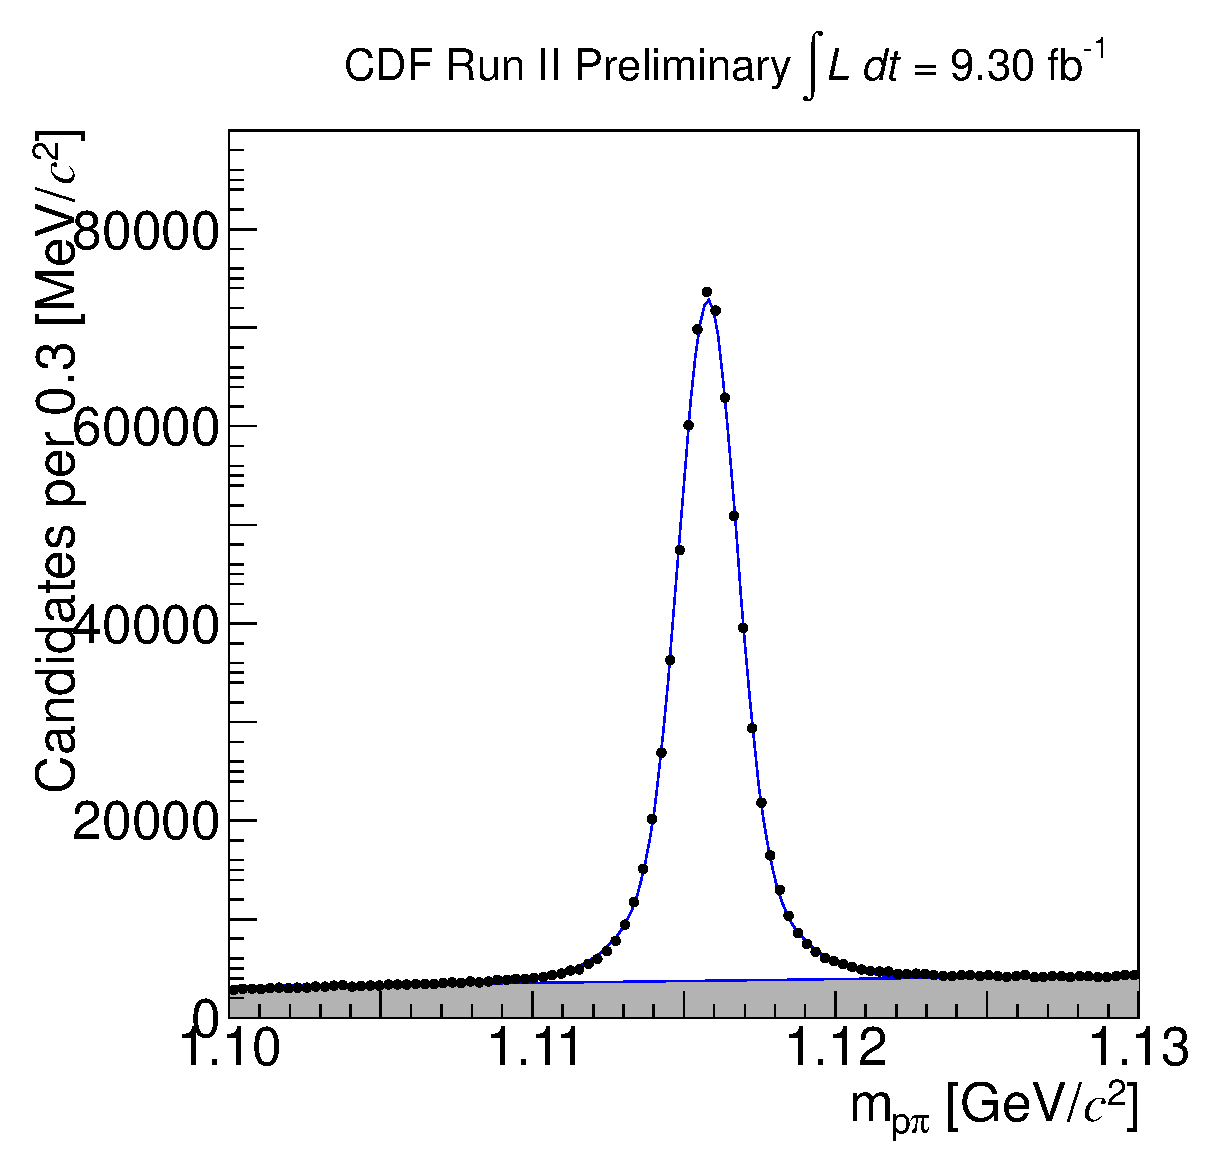
\includegraphics[scale=0.34]{./fig/canvas_fit_AL.eps}
\hspace{0.6cm}
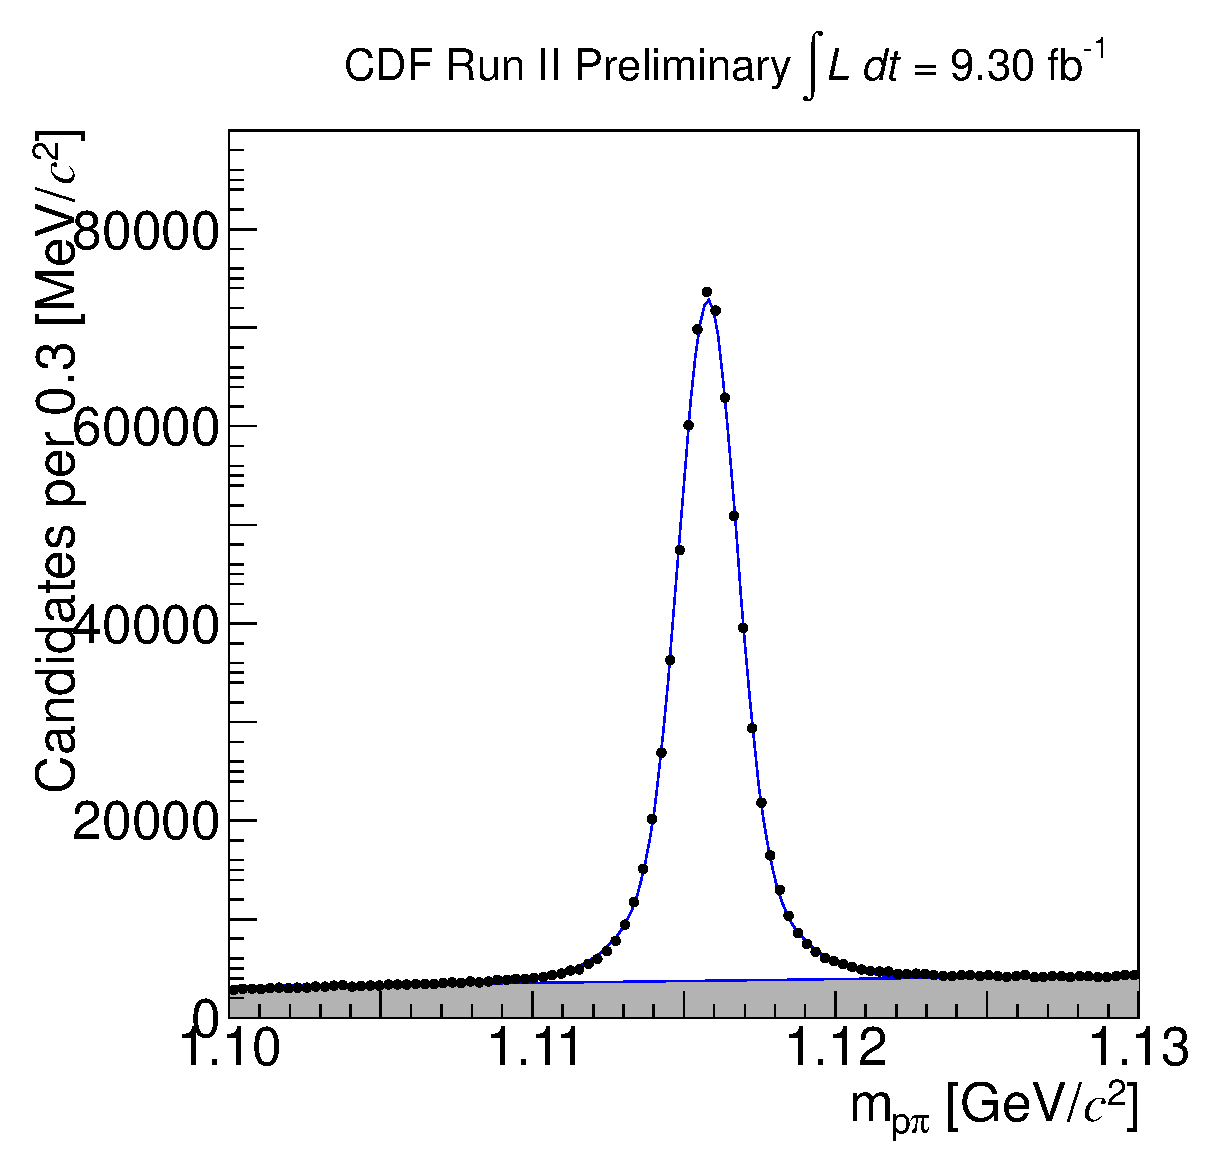
\includegraphics[scale=0.34]{./fig/canvas_fit_AL.eps}
\end{center}
\caption[Massa Invariante]{Dstribuzione della massa invariante in ipotesi $p\pi^-$ per i decadimenti 
\lambdazeroppi\ (a sinistra)  e  della massa invariante in ipotesi  $\bar{p}\pi^{+}$ per i decadimenti \alambdazeroppi\ (a destra).}
\label{fig:massa_invariante2}
\end{figure}
%%%%%%%%%%%%%%%%%%%%%%%%%%%%%%%%%%%%


%%%%%%%%%%%%%%%%%%%%%%%%%%%%%%%%%%%%%%%%%%%%%%%%%%%%%%%%%%%%%%%%%%%%%%%%%%%%%%%%
%%%%%%%%%%%%%%%%%%%%%%%%%%%%%%%%%%%%%%%%%%%%%%%%%%%%%%%%%%%%%%%%%%%%%%%%%%%%%%%%
%%%%%%%%%%%%%%%%%%%%%%%%%%%%%%%%%%%%%%%%%%%%%%%%%%%%%%%%%%%%%%%%%%%%%%%%%%%%%%%%


\section{Tabelle}
\label{sec:tabelle}

Questa sezione mostra invece come inserire delle tabelle nel testo (e altre equazioni come in sezione~\ref{sec:equazioni}). 
Tab.~\ref{tab:selezione} riporta le richieste offline utilizzate per selezionare 
il campione di dati mostrato in fig.~(\ref{fig:massa_invariante}).
%%%%%%%%%%%%%%%%%%%%%%%%%%%%%%%%%%%%%%%%%%%%%%%%%%%%%%%%%%%%
%%% Tabella dei tagli trigger confirmation %%%%%%%%%%%%%%%%%
%%%%%%%%%%%%%%%%%%%%%%%%%%%%%%%%%%%%%%%%%%%%%%%%%%%%%%%%%%%%
\begin{table}[!ht]
\centering
\begin{tabular}{lcc}
\hline\hline
Variabile della traccia		        &	Unit\`a		&	Richiesta		\\
\hline						                                                
$\pt(p)$ 						&	\pgev\		&	$>2.0$			\\
$|\eta(p)|$					&	$-$                  &	$<1.0$			\\
$|d_0(p)|$ 				        &    \mum\		&	$[100,~1000]$		\\
\hline
Variabile del candidato      		&         			&			           	\\
\hline
$q(p)\times q(\pi)$				&	$e^2$		&	$-1$			\\
$d_0(p) \times d_0(\pi)$			&	$\mum^2$	&	$< 0$			\\
\lxy\ 						&	 cm		        &	$[0.5,2.2]$		\\
$|z_{0}(p)-z_{0}(\pi)|$	 		&	 cm		        &	$<2$			\\
$m_{p\pi}$						&	\massgev	&	$[1.10,~1.13]$		\\
\hline\hline
\end{tabular}
\caption[Off-line selection for $\Lambda^0\to p\pi^-$]{Sommario della selezione utilizzata per ricostruire 
il campione di decadimenti \lambdazeroppi.
}  
\label{tab:selezione}
\end{table} 
%
%
L'asimmetria di carica indotta dal rivelatore nei decadimenti \lambdazeroppi\  pu\`o essere determinata 
attraverso un fit binnato simultaneo  di minimo  $\chi^2$  dei campioni di dati dei decadimenti \lambdazeroppi\ e
\alambdazeroppi. 
La distribuzione della densit\`a di probabilit\`a  (p.d.f) della massa invariante  per il segnale \`e parametrizzata attraverso 
una doppia gaussiana:
\begin{eqnarray}
\pdf_{s} = f \cdot \mathcal{G}(m;\mu_1, \sigma_{1} ) + (1 - f)\cdot \mathcal{G}(m;\mu_2, \sigma_{2} ),
\end{eqnarray}
dove il simbolo $\mathcal{G}$ indica la distribuzione Gaussiana normalizzata
\begin{eqnarray}
\mathcal{G}(m;\mu, \sigma ) & = & \frac{1}{\sqrt{2\pi\sigma^{2}}} e^{-\frac{1}{2}\left( \frac{m-\mu}{\sigma} \right)^{2}},
\end{eqnarray}
dove $\mu_1$ e  $\mu_2$  (con $\mu_1=\mu_2=\mu$) sono le medie delle due Gaussiane, $\sigma_1$ e $\sigma_2$ sono le 
deviazioni standard, e $f$ \`e la frazione relativa tra le due.
La p.d.f. della massa invariante per il fondo combinatorio \`e parametrizzata utilizzando una funzione esponenziale:
\begin{eqnarray}
\pdf_{b} =  \frac{e^{\lambda m}}{ \int_{a}^{b} e^{\lambda m} dm} %\mathcal{E}(m;\lambda ) 
\end{eqnarray}
dove $a=1.10~\massgev$ e $b=1.13~\massgev$ sono gli estremi di integrazione e quindi del dominio in cui viene 
effettutato il fit simultaneo, e $\lambda$ \`e la pendenza dell'esponenziale che viene determinata dal fit.
%\begin{eqnarray}
%\mathcal{E}(m;\lambda )       & = & \frac{\cdot e^{\lambda m}}{ \int_{a}^{b}\cdot e^{\lambda m} dm}
%\end{eqnarray}
La p.d.f totale si scrive quindi come:
\begin{eqnarray}
\pdf_{\rm tot} = w\cdot \left(N_{s}\cdot \pdf_{s} + N_{b}\cdot \pdf_{b}\right)
\end{eqnarray}
dove $w=0.3~\pmev$ \`e la larghezza del bin dei due istogrammi.
I campioni di dati dei decadimenti \lambdazero\ e \alambdazero\ vengono fittati simultaneamente e i risultati sono riportati in tab.~(\ref{tab:fit}).
\begin{table}[!ht]
\centering
\begin{tabular}{lccc}
\hline\hline
Parametro			&	\lambdazero\        				&	\alambdazero\			& Asymmetria (\%)		 \\
\hline				                                                	
N$_{s}$	                 	&	94235 $\pm$ 352 			        &	92075  $\pm$ 349           	& 0.012 $\pm$  0.003	\\
$N_{b}$		         	& 	48748 $\pm$ 278				& 	48906 $\pm$ 277	                & -0.002 $\pm$ 0.004  \\
$f$					& 	\multicolumn{2}{c}{0.336 $\pm$ 0.015}		&   combinato \\
$\mu$				& 	1.11578 $\pm$ 0.000004		& 1.11578 $\pm$ 0.000004	       & -0.000006 $\pm$ 0.000003 \\
$\sigma_{1}$			& 	\multicolumn{2}{c}{0.00189 $\pm$ 0.00004}	 	& combinato\\
$\sigma_{2}$			& 	\multicolumn{2}{c}{0.00092 $\pm$ 0.00001}		& combinato\\
$\lambda$	         	& 	\multicolumn{2}{c}{11.30 $\pm$ 0.37}			 	& combinato\\
\hline\hline
\end{tabular}
\caption[Results of the fit]{Risultati del fit simultaneo.}
\label{tab:fit}
\end{table} 
Le proiezioni del fit sulle distribuzioni di  massa invariante sono riportate in fig.~(\ref{fig:massa_invariante}).
Il valore raw dell'asimmetria misurato dal fit \`e:
\begin{equation}
A^{\rm raw}=\frac{\mathcal{N}(\lambdazeroppi) - \mathcal{N}(\alambdazeroppi)}{\mathcal{N}(\lambdazeroppi) + \mathcal{N}(\alambdazeroppi)} =  (1.2 \pm  0.3)\%     %9fb/1
\label{eq:asym_raw_result}
\end{equation}
dove l'incertezza \`e solo di origine statistica.  Il risultato ottenuto \`e in accordo con 
la misura precedente di (0.72 $\pm$ 0.53)\% di Ref.~\cite{prl_acp}, in cui una tecnica sperimentale simile
\`e stata utilizzata per estrarre la stessa asimmetria di carica.   Maggiori dettagli possono essere trovati 
in \cite{Aad:2012tfa,Chatrchyan:2012ufa}. 

Un utile manuale in rete del linguaggio \latex\ si trova in \cite{manuale_latex}. I dettagli degli innumerevoli pacchetti
che possono essere utilizzati si trovano nel ``The Comprehensive \TeX\ Archive Network''~\cite{ctan}.




%\appendix


\begin{thebibliography}{99}

\bibitem{prl_acp}
T. Aaltonen et al. (CDF Collaboration), \textit{Measurements of Direct CP 
Violating Asymmetries in Charmless Decays of Strange Bottom Mesons and Bottom Baryons},
Phys. Rev. Lett. {\bf 106}, 181802 (2011), arXiv:1103.5762 [hep-ex].

\bibitem{Aad:2012tfa}
G. Aad et al. (ATLAS Collaboration) \textit{Observation of a new particle in the search for the Standard 
Model Higgs boson with the ATLAS detector at the LHC}, Phys.Lett. {\bf B716}, 1-29 (2012), arXiv:1207.7214 [hep-ex].

\bibitem{Chatrchyan:2012ufa}
S. Chatrchyan et al. (CMS Collaboration), \textit{Observation of a new boson at a mass of 125 GeV with the CMS experiment at the LHC},
Phys.Lett. {\bf B716}, 30-61 (2012), arXiv:1207.7235 [hep-ex].

\bibitem{manuale_latex} {\tt http://www.lorenzopantieri.net/LaTeX\_files/ArteLaTeX.pdf}

\bibitem{ctan} {\tt http://www.ctan.org/}

\end{thebibliography}


\end{document}